\subsection{Mobility}
As \ues traverse the \xcloud network, the service(s) they subsribe to will migrate accordingly to accomodate the changeing distribution of \ues. The 2-dimensional, multi modal, mobility model detailed in \cite{bettstetter2001smooth} provides us with a uniform distribution of users, with a realistic rate of mobility, see Figure \ref{fig:mobility_distribution}.

\begin{figure}[tb]
	\centering
	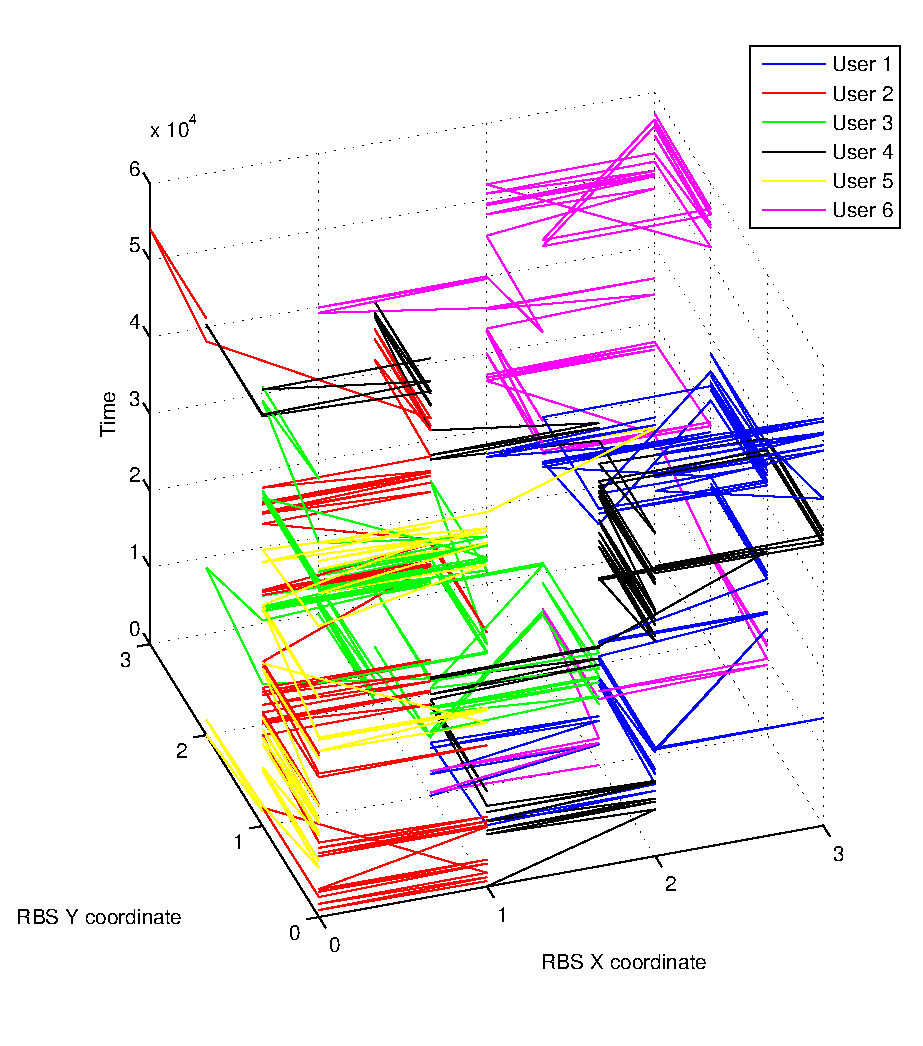
\includegraphics[width=\linewidth]{user_mobility.eps} 
	\caption{\Ue mobility between \rbs over time}
	\label{fig:mobility_distribution}
\end{figure}

The model defines the fundamental timeing and mobility properties \ue movement, such as the speed, acceleration, and direction the \ue is moving in, as well as for how long and when next to turn. 